Molto bene la presenza di una ricerca globale nel sito. L'utente, infatti, apprezza moltissimo questa soluzione e, se presente, la usa sempre.

\paragraph*{Implementazione}
Molto bene. \`E una semplice barra con un pulsante cerca, che compare quando si clicca sulla lente di ingrandimento. Non sono presenti ulteriori opzioni che confonderebbero solamente l'utente.

\begin{figure}
	\centering
	
\includegraphics[width=\textwidth]{sez/Elementi_Comuni/img/barra_ricerca.png}
	\caption{Barra di ricerca}
	\label{fig:barra_ricerca}
\end{figure}

\paragraph*{Risultati di ricerca}
I risultati vengono presentati in una lista in stile Google molto familiare all'utente. Non benissimo i soliti link \textit{"Clicca qui per andare a pagina X"}. Bene anche la ricerca senza risultati, che viene correttamente segnalata all'utente. Non sono presenti ulteriori filtri per la ricerca (ma non sono nemmeno necessari). Altri piccoli difetti si notano nel numero di risultati della query in lingua inglese (\autoref{fig:pagina_ricerca}) e nel testo troppo largo e difficile da leggere.

\begin{figure}[H]
	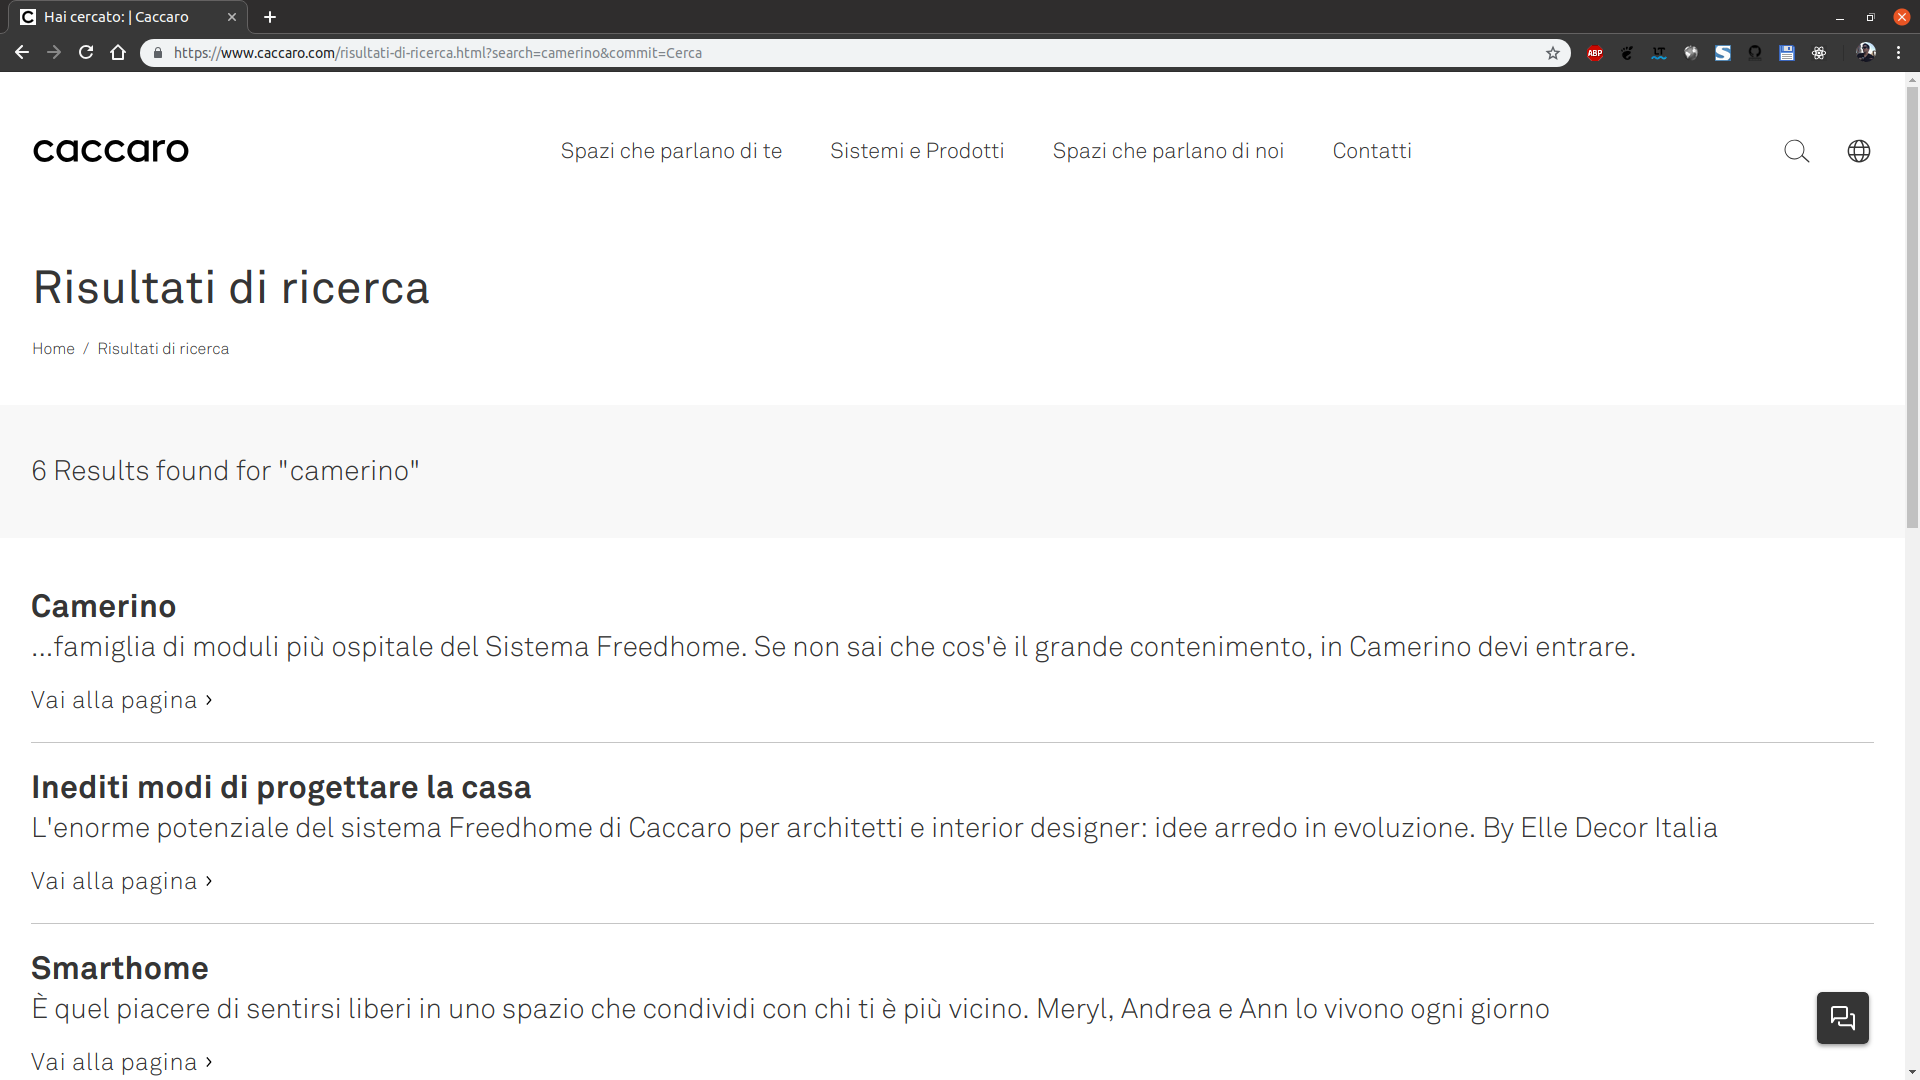
\includegraphics[width=\textwidth]{sez/Elementi_Comuni/pag_ricerca.png}
	\caption{Pagina di ricerca.}
	\label{fig:pagina_ricerca}
\end{figure}